% !TEX program = xelatex
\documentclass[12pt,a4paper]{article}

% =================== PACKAGES ===================
\usepackage[T1]{fontenc}
\usepackage{geometry}
\usepackage{graphicx}
\usepackage{hyperref}
\usepackage{enumitem}
\usepackage{titlesec}
\usepackage{fancyhdr}
\usepackage{booktabs}
\usepackage{array}
\usepackage{tabularx}
\usepackage{setspace}
\usepackage[final,nopatch=footnote]{microtype}
\usepackage{newtxtext}
\usepackage{parskip}
\usepackage[nottoc]{tocbibind}
\usepackage{tikz}
\usetikzlibrary{arrows.meta, positioning, shapes.geometric, backgrounds, calc, fit, matrix}
\usepackage{caption}
\captionsetup{font=small, labelfont=bf, margin=0.5cm}
\usepackage{float}
\usepackage{xcolor}
\usepackage{pdflscape}
\usepackage{ragged2e}
\graphicspath{{/Users/krust/Documents/eaClass/Seminar2/}}

% =================== PAGE LAYOUT ===================
\geometry{
  top=1in,
  bottom=1in,
  left=1.05in,
  right=1.05in,
  headheight=14pt,
  headsep=18pt
}
\setstretch{1.12}
\setlength{\emergencystretch}{2em}

% =================== COLOURS ===================
\definecolor{lkblue}{HTML}{1F5B8F}
\definecolor{lkcyan}{HTML}{E9F4FB}
\definecolor{lkgreen}{HTML}{2E7D32}
\definecolor{lkorange}{HTML}{C46A1A}
\definecolor{lkpurple}{HTML}{6A4C93}
\definecolor{lkgray}{HTML}{F4F6F8}
\definecolor{darkgray}{HTML}{333333}

% =================== HEADER / FOOTER ===================
\pagestyle{fancy}
\fancyhf{}
\fancyhead[L]{\small IK2015 \textemdash{} Enterprise Architecture and Database Programming}
\fancyhead[R]{\small Seminar 2: BSC and Business Model Canvas}
\fancyfoot[C]{\thepage}
\renewcommand{\headrulewidth}{0.4pt}

% =================== SECTION FORMATTING ===================
\titleformat{\section}[hang]{\Large\bfseries\color{darkgray}}{\thesection}{1em}{}
\titleformat{\subsection}[hang]{\large\bfseries\color{darkgray}}{\thesubsection}{1em}{}
\titlespacing*{\section}{0pt}{12pt}{6pt}
\titlespacing*{\subsection}{0pt}{10pt}{4pt}

% =================== HYPERLINK SETUP ===================
\hypersetup{
  colorlinks=true,
  linkcolor=black,
  citecolor=black,
  urlcolor=lkblue,
  pageanchor=false
}

% =================== TABLE HELPERS ===================
\newcolumntype{Y}{>{\RaggedRight\arraybackslash}X}
\newcolumntype{P}[1]{>{\RaggedRight\arraybackslash}p{#1}}
\renewcommand{\arraystretch}{1.28}
\newcommand{\landscapepagenumber}{\vfill\begin{center}\thepage\end{center}}

% =================== TITLE AREA ===================
\title{}
\author{}
\date{}

\begin{document}

% ---- Custom Title Page ----
\thispagestyle{empty}
\vspace*{1.8cm}

\begin{center}
  {\normalsize Jiangxi University of Finance and Economics} \\[2.1cm]

  {\LARGE\bfseries Balanced Scorecard and Business Model Canvas Report} \\[1.0cm]

  {\Large Luckin Coffee Inc.} \\[0.25cm]
  {\normalsize\itshape A Technology-Driven New Retail Coffee Enterprise} \\[2.0cm]

  {\normalsize IK2015: Enterprise Architecture and Database Programming} \\[0.2cm]
  {\normalsize Seminar 2} \\[2.2cm]

  {\normalsize\textbf{Group 4}} \\[0.45cm]
  {\normalsize
    Zhe-Kai Yang~(Krust),\quad
    Shi-Hang Chen~(Sean),\quad
    Wei-Yu Cai~(Nosta), \\[0.2cm]
    Huan-Wen Chen~(Evan),\quad
    Yuan-Yong Liao~(Foreve)
  } \\[1.8cm]

  {\normalsize \today}
\end{center}

\newpage
\hypersetup{pageanchor=true}
\setcounter{page}{1}
\pagenumbering{arabic}
\pagestyle{fancy}

% =================== BASIC INFORMATION ===================
\section{Report Basic Information}

\begin{table}[H]
\centering
\caption{Basic information of the selected case enterprise.}
\begin{tabularx}{\textwidth}{P{4.2cm}Y}
\toprule
\textbf{Item} & \textbf{Information} \\
\midrule
Selected enterprise / business & Luckin Coffee Inc.; technology-enabled coffee retail, pickup, delivery, and packaged coffee business. \\
Course and seminar & IK2015 Enterprise Architecture and Database Programming; Seminar 2. \\
Group number & Group 4. \\
Group members & \parbox[t]{\hsize}{\raggedright Zhe-Kai Yang~(Krust), Shi-Hang Chen~(Sean), Wei-Yu Cai~(Nosta),\\ Huan-Wen Chen~(Evan), Yuan-Yong Liao~(Foreve).} \\
Analytical frameworks & Balanced Scorecard and Business Model Canvas. \\
\bottomrule
\end{tabularx}
\end{table}

Luckin Coffee is selected as the case enterprise because its business model combines physical store operations, mobile-first ordering, digital payment, delivery coordination, franchise-style partnership stores, supply chain integration, and data-driven customer relationship management. These elements are tightly coupled in daily operations, making the company a suitable case for enterprise architecture analysis: strategic objectives, operational processes, information systems, and measurable performance indicators are all directly observable in its routine business activities.

% =================== CASE SNAPSHOT ===================
\section{Case Enterprise Snapshot}

Luckin Coffee Inc. was founded in 2017 and is headquartered in Xiamen, China. Its strategic positioning differs from the traditional premium caf\'{e} model. Rather than relying on store ambience and long in-store consumption time, Luckin emphasises affordable products, dense store coverage, mobile ordering, rapid pickup, and delivery convenience. According to its public filings and investor disclosures, the corporate mission is ``to create lucky moments and inspire,'' and the vision is ``to build a world-class coffee brand and become a part of everyone's daily life''~\cite{luckin2025annual}. This mission reflects a mass-market strategy: coffee is treated as a daily routine product rather than an occasional luxury.

\begin{figure}[H]
  \centering
  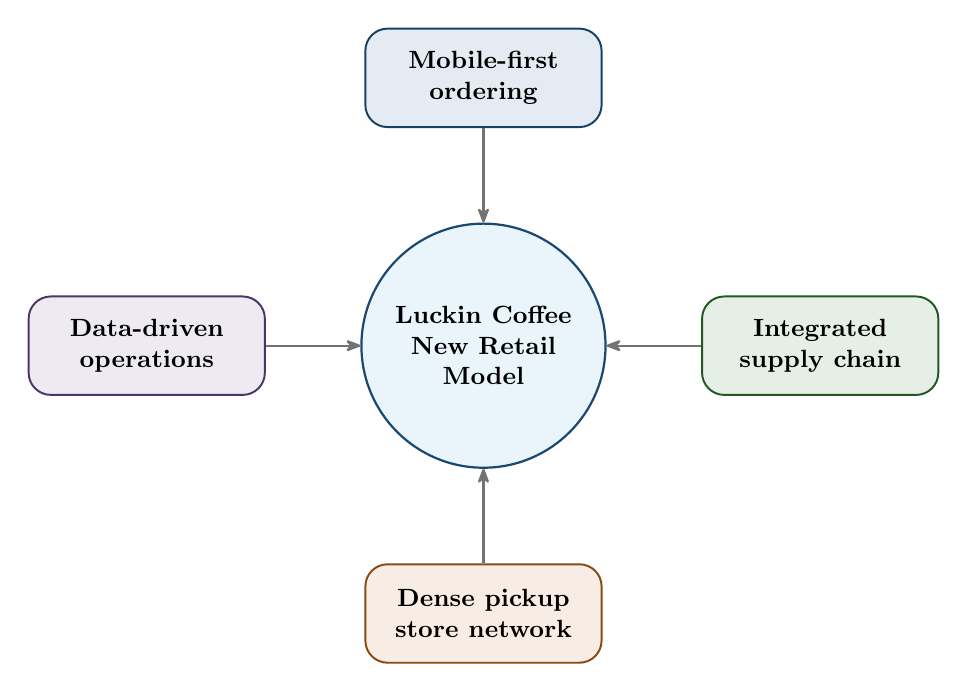
\begin{tikzpicture}[
    node distance=1.2cm,
    pillar/.style={rectangle, rounded corners=8pt, draw=#1!70!black, fill=#1!12,
                   minimum width=3.0cm, minimum height=1.25cm, align=center,
                   font=\small\bfseries, line width=0.7pt},
    center/.style={circle, draw=lkblue!80!black, fill=lkcyan, minimum size=3.1cm,
                   align=center, font=\small\bfseries, line width=0.8pt},
    arrow/.style={-{Stealth[round]}, line width=0.8pt, black!55}
  ]
    \node[center] (core) {Luckin Coffee\\New Retail\\Model};
    \node[pillar=lkblue, above=of core] (digital) {Mobile-first\\ordering};
    \node[pillar=lkgreen, right=of core] (supply) {Integrated\\supply chain};
    \node[pillar=lkorange, below=of core] (stores) {Dense pickup\\store network};
    \node[pillar=lkpurple, left=of core] (data) {Data-driven\\operations};

    \draw[arrow] (digital) -- (core);
    \draw[arrow] (supply) -- (core);
    \draw[arrow] (stores) -- (core);
    \draw[arrow] (data) -- (core);
  \end{tikzpicture}
  \caption{Strategic logic of Luckin Coffee's new retail model.}
\end{figure}

The enterprise reported rapid growth in recent years, supported by a hybrid network of self-operated stores and partnership stores. Its revenue model combines direct sales from self-operated stores with franchise-related income, raw material and equipment sales, delivery charges, and packaged coffee sales~\cite{luckin2025annual,luckin2025results}. The following sections translate this business logic into two complementary frameworks: the Balanced Scorecard and the Business Model Canvas.

% =================== BSC ===================
\section{Balanced Scorecard Analysis}

The Balanced Scorecard translates strategy into a structured set of missions, objectives, and performance measures across four perspectives: financial, customer, internal process, and learning and growth. For Luckin Coffee, these perspectives are mutually reinforcing. Financial performance depends on customer retention and store productivity; customer experience depends on fast digital ordering and stable product quality; internal processes depend on integrated systems and supply chain discipline; and long-term growth depends on product innovation, employee capability, and data infrastructure.

\subsection{Strategy Map}

\begin{figure}[H]
  \centering
  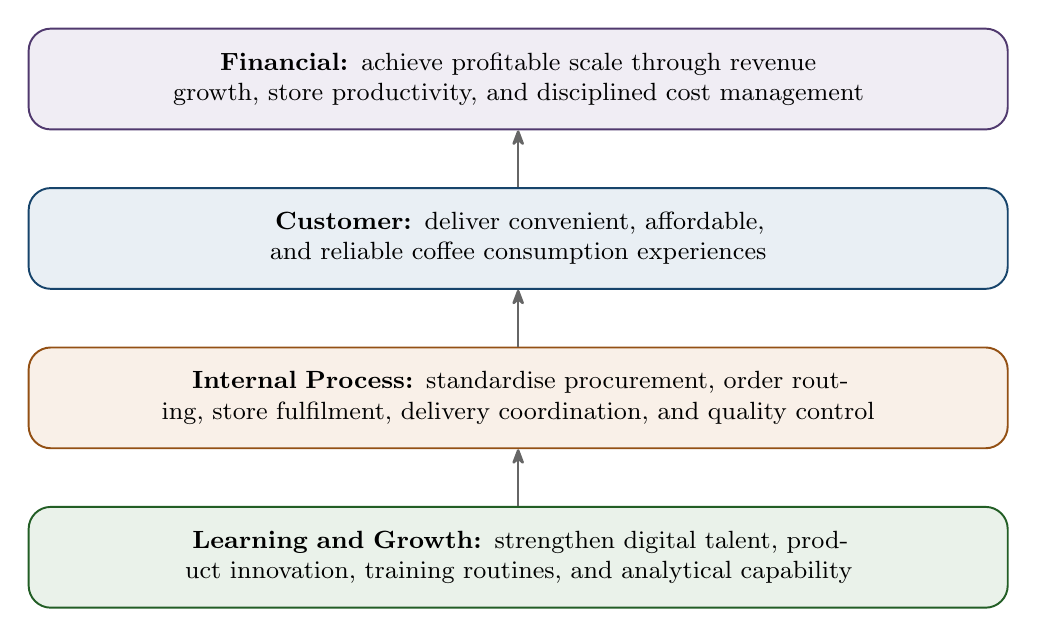
\begin{tikzpicture}[
    layer/.style={rectangle, rounded corners=8pt, draw=#1!75!black, fill=#1!10,
                  text width=12.2cm, minimum height=1.28cm, align=center,
                  font=\small, line width=0.7pt},
    labelbox/.style={rectangle, rounded corners=5pt, draw=#1!75!black, fill=#1!18,
                     text width=3.2cm, minimum height=0.8cm, align=center,
                     font=\footnotesize\bfseries},
    arrow/.style={-{Stealth[round]}, line width=0.9pt, black!60}
  ]
    \node[layer=lkgreen] (learn) {\textbf{Learning and Growth:} strengthen digital talent, product innovation, training routines, and analytical capability};
    \node[layer=lkorange, above=0.72cm of learn] (process) {\textbf{Internal Process:} standardise procurement, order routing, store fulfilment, delivery coordination, and quality control};
    \node[layer=lkblue, above=0.72cm of process] (customer) {\textbf{Customer:} deliver convenient, affordable, and reliable coffee consumption experiences};
    \node[layer=lkpurple, above=0.72cm of customer] (financial) {\textbf{Financial:} achieve profitable scale through revenue growth, store productivity, and disciplined cost management};

    \draw[arrow] (learn) -- (process);
    \draw[arrow] (process) -- (customer);
    \draw[arrow] (customer) -- (financial);
  \end{tikzpicture}
  \caption{Balanced Scorecard strategy map for Luckin Coffee.}
\end{figure}

\subsection{Balanced Scorecard Table}

\begin{landscape}
\thispagestyle{empty}
\begin{table}[H]
\centering
\scriptsize
\renewcommand{\arraystretch}{1.12}
\caption{Balanced Scorecard for Luckin Coffee.}
\begin{tabularx}{\linewidth}{P{2.7cm}P{5.1cm}P{8.2cm}Y}
\toprule
\textbf{Perspective} & \textbf{Mission} & \textbf{Objectives} & \textbf{Directly Related Measures} \\
\midrule
\textbf{Financial} &
Build a scalable and profitable coffee retail platform while maintaining affordability for mass-market customers. &
\begin{enumerate}[leftmargin=*,nosep]
  \item Increase total net revenue through store expansion, higher purchase frequency, and packaged coffee sales.
  \item Improve store-level profitability by balancing self-operated control with partnership-store expansion.
  \item Maintain cost discipline in raw materials, rent, labour, logistics, and promotional spending.
\end{enumerate} &
\begin{enumerate}[leftmargin=*,nosep]
  \item Total net revenue, year-on-year revenue growth rate, same-store sales growth, and packaged coffee sales revenue.
  \item Store-level operating margin, average order value, and revenue split between self-operated stores and partnership stores.
  \item Raw material cost ratio, rent and labour cost ratio, logistics cost per order, and promotional expense ratio.
\end{enumerate} \\
\midrule
\textbf{Customer} &
Make coffee a convenient, affordable, and habitual part of everyday life for urban consumers. &
\begin{enumerate}[leftmargin=*,nosep]
  \item Increase customer retention and repeat purchase frequency through digital membership and targeted promotions.
  \item Improve perceived convenience through fast pickup, reliable delivery, and dense store coverage.
  \item Strengthen brand trust by ensuring stable taste, quality, hygiene, and service consistency.
\end{enumerate} &
\begin{enumerate}[leftmargin=*,nosep]
  \item Monthly average transacting customers, active membership users, repeat purchase rate, and customer lifetime value.
  \item Average pickup time, delivery completion time, nearby-store coverage, and order cancellation rate.
  \item Customer rating, complaint rate, product quality complaint rate, and net promoter score.
\end{enumerate} \\
\midrule
\textbf{Internal Processes} &
Operate a tightly integrated digital-to-physical value chain from demand forecasting to store fulfilment. &
\begin{enumerate}[leftmargin=*,nosep]
  \item Standardise procurement, production, fulfilment, and quality-control routines across self-operated and partnership stores.
  \item Use data systems to improve demand forecasting, inventory replenishment, and labour scheduling.
  \item Reduce operational friction in app ordering, payment, order routing, and after-sales feedback.
\end{enumerate} &
\begin{enumerate}[leftmargin=*,nosep]
  \item Store audit pass rate, recipe compliance rate, order fulfilment accuracy, and product quality consistency indicators.
  \item Forecast accuracy, inventory turnover, stockout rate, raw material wastage rate, and labour utilisation rate.
  \item System uptime, app transaction success rate, order-routing error rate, and average response time for customer feedback.
\end{enumerate} \\
\midrule
\textbf{Learning and Growth} &
Develop organisational capabilities that support rapid innovation, digital operations, and sustainable expansion. &
\begin{enumerate}[leftmargin=*,nosep]
  \item Improve employee training, standard operating procedure compliance, and store-manager capability.
  \item Accelerate product innovation by using sales data, consumer feedback, and regional taste preferences.
  \item Strengthen data governance, analytics capability, and technology platform resilience.
\end{enumerate} &
\begin{enumerate}[leftmargin=*,nosep]
  \item Training completion rate, employee productivity, employee turnover rate, and store-manager assessment results.
  \item Number of new products launched, new-product success rate, product iteration cycle time, and customer feedback adoption rate.
  \item Data accuracy, dashboard adoption, analytics-supported decision rate, IT investment intensity, and critical incident resolution time.
\end{enumerate} \\
\bottomrule
\end{tabularx}
\end{table}
\landscapepagenumber
\end{landscape}

The proposed indicators are organised so that each measure directly tests the objective with the same number. For example, the third financial objective concerns cost discipline, so its related measures focus on raw material cost ratio, rent and labour cost ratio, logistics cost per order, and promotional expense ratio. This structure makes the link between mission, objectives, and measures clearer: the mission states the strategic intention, the objectives describe what must be achieved, and the measures show how achievement can be checked. Performance management, as the Balanced Scorecard framework argues, should connect financial results to the operational drivers that produce them rather than defaulting to short-term financial accounting.

\begin{figure}[H]
  \centering
  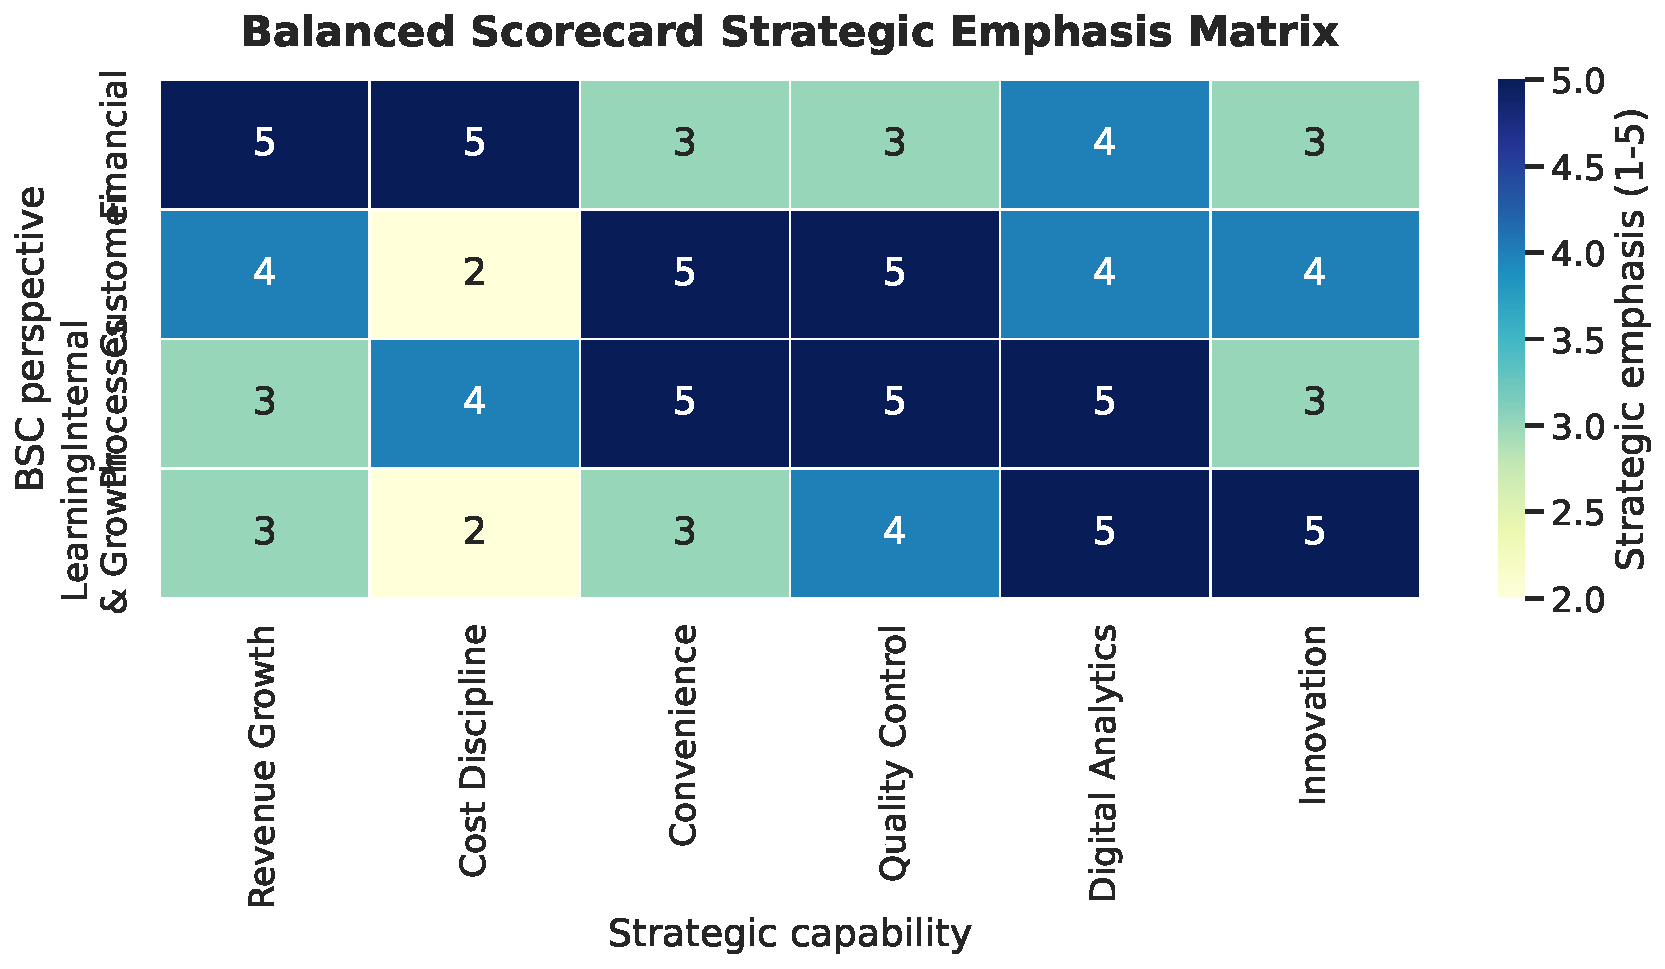
\includegraphics[width=0.90\textwidth]{fig_bsc_heatmap.pdf}
  \caption{Analytical heatmap of strategic emphasis across the Balanced Scorecard. Scores are qualitative assessments derived from the Luckin Coffee case analysis.}
\end{figure}

The heatmap shows that financial performance is most strongly associated with revenue growth and cost discipline; customer performance with convenience and quality control; internal processes with fulfilment reliability and digital analytics; and learning and growth with innovation and data capability. This pattern is consistent with Luckin's technology-enabled retail logic, where digital infrastructure supports both operational control and market responsiveness.

% =================== BUSINESS MODEL CANVAS ===================
\section{Business Model Canvas}

The Business Model Canvas provides a compact view of how Luckin Coffee creates, delivers, and captures value. The central value proposition extends beyond the coffee product itself: customers choose products, receive promotions, pay, and decide between pickup and delivery through a mobile interface — convenience is the core offering, with coffee as the carrier. The canvas below maps this logic into the nine standard components.

\begin{landscape}
\thispagestyle{empty}
\begin{figure}[H]
\centering
\footnotesize
\resizebox{0.985\linewidth}{!}{%
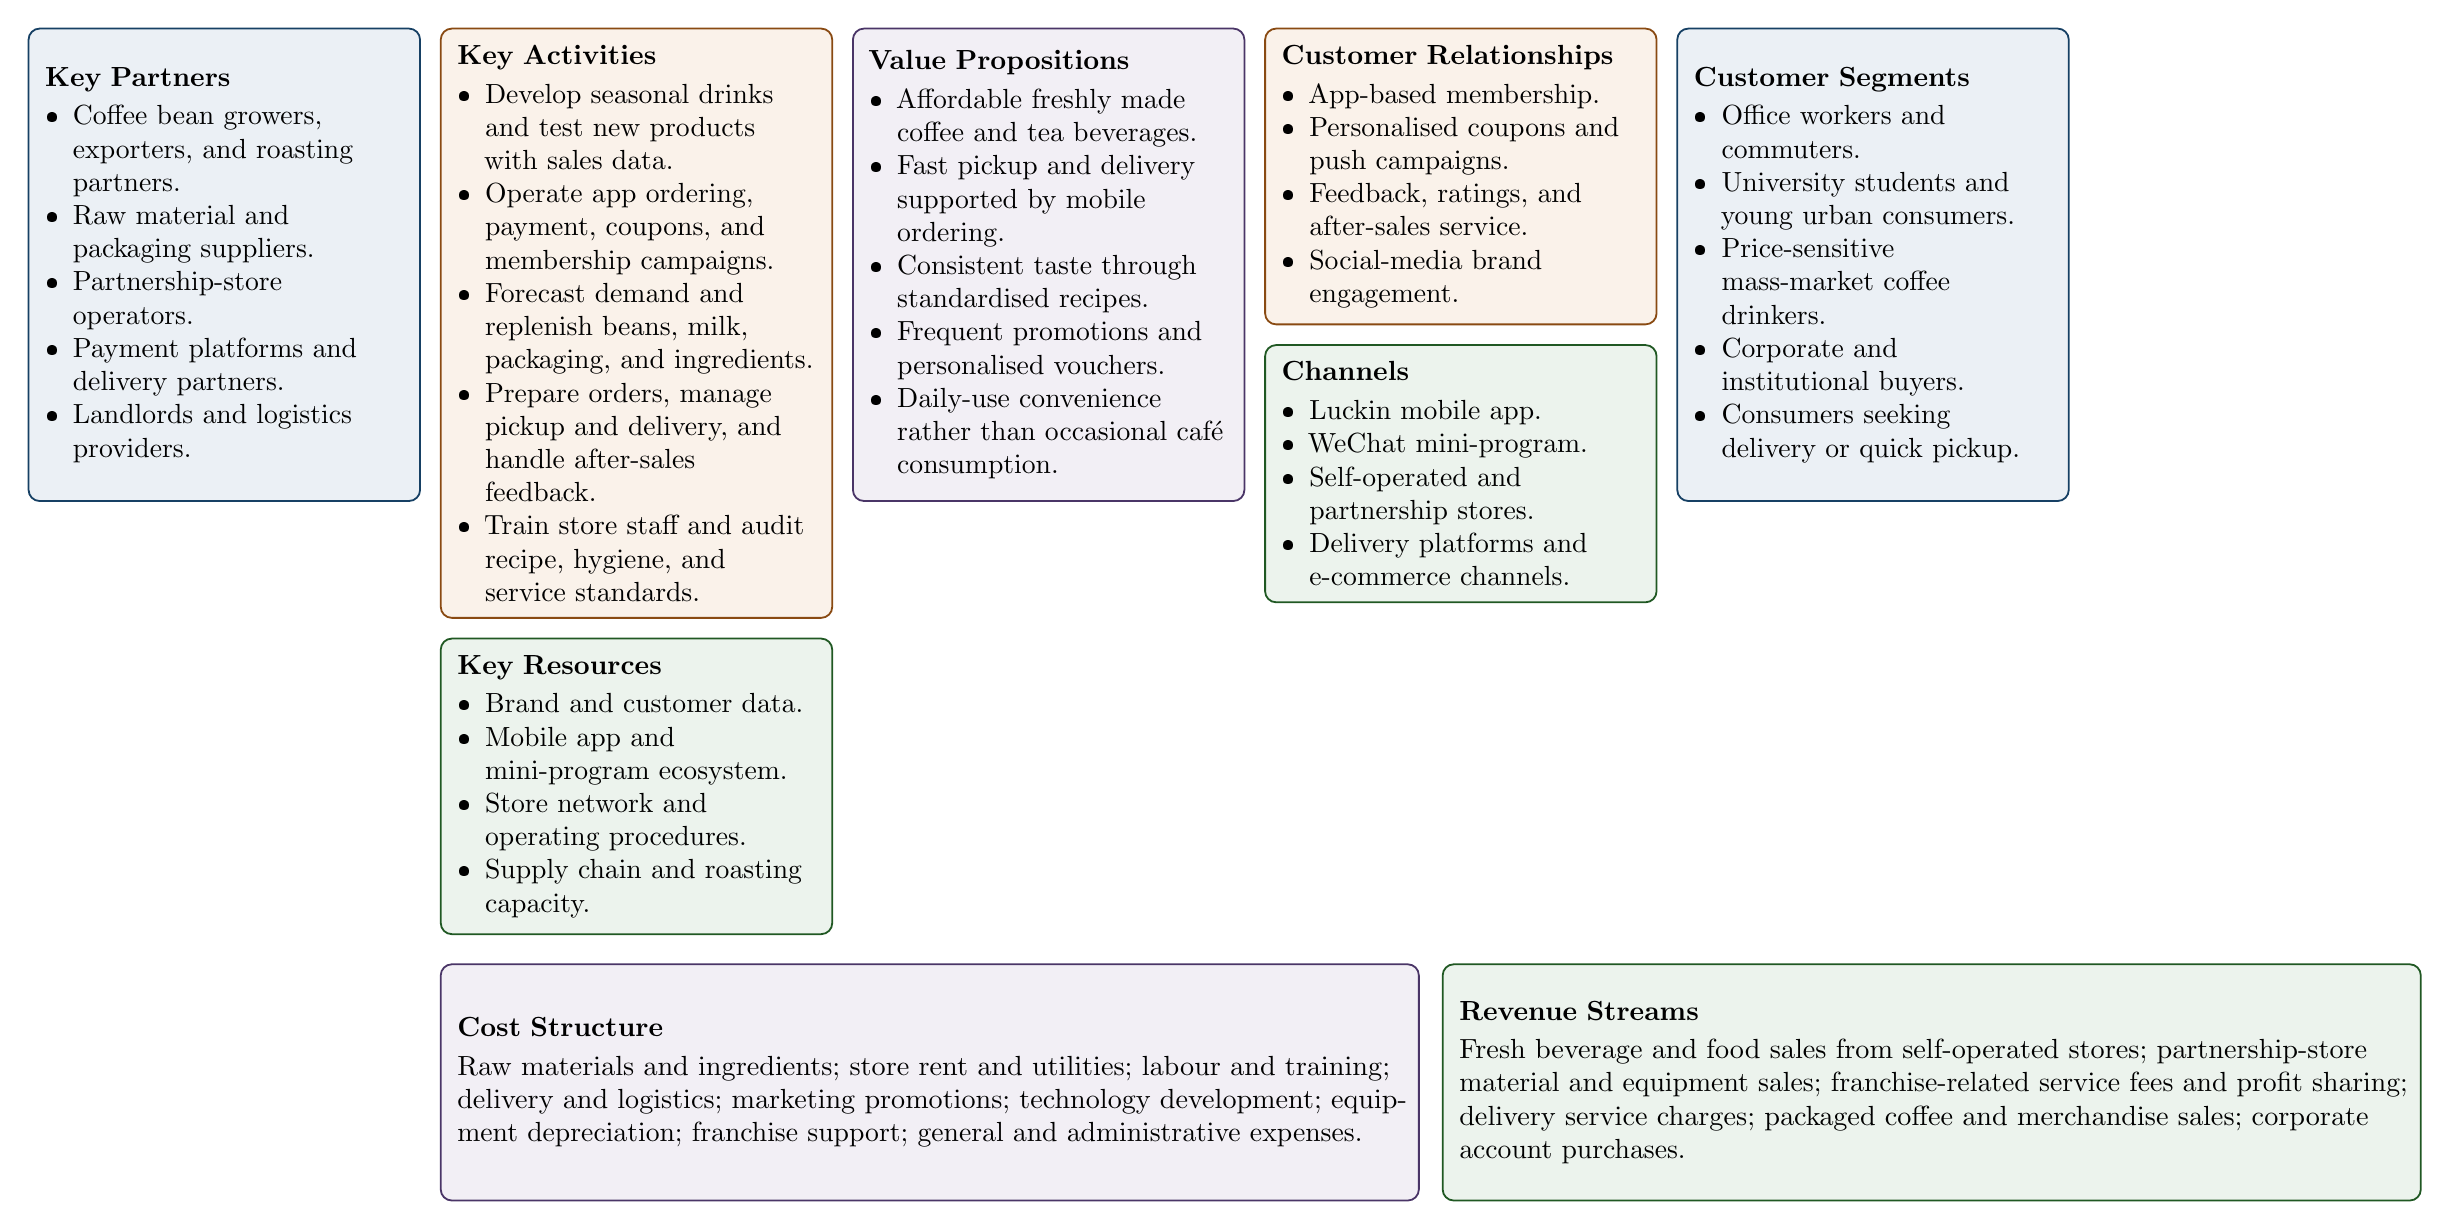
\begin{tikzpicture}[
  canvasbox/.style={rectangle, draw=#1!70!black, fill=#1!9, rounded corners=4pt,
                    text width=4.55cm, minimum height=6.0cm, align=left, inner sep=6pt, line width=0.65pt},
  smallbox/.style={rectangle, draw=#1!70!black, fill=#1!9, rounded corners=4pt,
                   text width=4.55cm, minimum height=2.9cm, align=left, inner sep=6pt, line width=0.65pt},
  widebox/.style={rectangle, draw=#1!70!black, fill=#1!9, rounded corners=4pt,
                  text width=11.6cm, minimum height=3.0cm, align=left, inner sep=6pt, line width=0.65pt},
  title/.style={font=\bfseries\color{darkgray}}
]
  \node[canvasbox=lkblue] (partners) at (0,0) {\textbf{Key Partners}\par\vspace{2pt}
    \begin{itemize}[leftmargin=*,nosep]
      \item Coffee bean growers, exporters, and roasting partners.
      \item Raw material and packaging suppliers.
      \item Partnership-store operators.
      \item Payment platforms and delivery partners.
      \item Landlords and logistics providers.
    \end{itemize}};

  \node[smallbox=lkorange, right=0.24cm of partners.north east, anchor=north west] (activities) {\textbf{Key Activities}\par\vspace{2pt}
    \begin{itemize}[leftmargin=*,nosep]
      \item Develop seasonal drinks and test new products with sales data.
      \item Operate app ordering, payment, coupons, and membership campaigns.
      \item Forecast demand and replenish beans, milk, packaging, and ingredients.
      \item Prepare orders, manage pickup and delivery, and handle after-sales feedback.
      \item Train store staff and audit recipe, hygiene, and service standards.
    \end{itemize}};

  \node[smallbox=lkgreen, below=0.24cm of activities] (resources) {\textbf{Key Resources}\par\vspace{2pt}
    \begin{itemize}[leftmargin=*,nosep]
      \item Brand and customer data.
      \item Mobile app and mini-program ecosystem.
      \item Store network and operating procedures.
      \item Supply chain and roasting capacity.
    \end{itemize}};

  \node[canvasbox=lkpurple, right=0.24cm of activities.north east, anchor=north west] (value) {\textbf{Value Propositions}\par\vspace{2pt}
    \begin{itemize}[leftmargin=*,nosep]
      \item Affordable freshly made coffee and tea beverages.
      \item Fast pickup and delivery supported by mobile ordering.
      \item Consistent taste through standardised recipes.
      \item Frequent promotions and personalised vouchers.
      \item Daily-use convenience rather than occasional caf\'{e} consumption.
    \end{itemize}};

  \node[smallbox=lkorange, right=0.24cm of value.north east, anchor=north west] (relationships) {\textbf{Customer Relationships}\par\vspace{2pt}
    \begin{itemize}[leftmargin=*,nosep]
      \item App-based membership.
      \item Personalised coupons and push campaigns.
      \item Feedback, ratings, and after-sales service.
      \item Social-media brand engagement.
    \end{itemize}};

  \node[smallbox=lkgreen, below=0.24cm of relationships] (channels) {\textbf{Channels}\par\vspace{2pt}
    \begin{itemize}[leftmargin=*,nosep]
      \item Luckin mobile app.
      \item WeChat mini-program.
      \item Self-operated and partnership stores.
      \item Delivery platforms and e-commerce channels.
    \end{itemize}};

  \node[canvasbox=lkblue, right=0.24cm of relationships.north east, anchor=north west] (segments) {\textbf{Customer Segments}\par\vspace{2pt}
    \begin{itemize}[leftmargin=*,nosep]
      \item Office workers and commuters.
      \item University students and young urban consumers.
      \item Price-sensitive mass-market coffee drinkers.
      \item Corporate and institutional buyers.
      \item Consumers seeking delivery or quick pickup.
    \end{itemize}};

  \node[widebox=lkpurple, below=0.36cm of resources.south west, anchor=north west, text width=12.0cm] (costs) {\textbf{Cost Structure}\par\vspace{2pt}
    Raw materials and ingredients; store rent and utilities; labour and training; delivery and logistics; marketing promotions; technology development; equipment depreciation; franchise support; general and administrative expenses.};

  \node[widebox=lkgreen, right=0.28cm of costs, text width=12.0cm] (revenues) {\textbf{Revenue Streams}\par\vspace{2pt}
    Fresh beverage and food sales from self-operated stores; partnership-store material and equipment sales; franchise-related service fees and profit sharing; delivery service charges; packaged coffee and merchandise sales; corporate account purchases.};
\end{tikzpicture}%
}
\caption{Business Model Canvas for Luckin Coffee.}
\end{figure}
\landscapepagenumber
\end{landscape}

\subsection{Interpretation of the Canvas}

Luckin's business model is essentially a platform-enabled retail system. Its physical stores are not isolated sales outlets; they are fulfilment nodes connected to a digital demand-generation and data-collection platform. The app and mini-program channels lower transaction friction, while the store network provides spatial proximity to customers. At the same time, customer data allows the company to design personalised promotions, forecast demand, evaluate new products, and refine site-level operations.

The canvas also reveals several strategic tensions. Affordability and frequent promotions support customer acquisition, but they compress margins when not offset by data-driven pricing and supply chain efficiency. Rapid expansion through partnership stores increases geographic coverage at the cost of quality and brand consistency risks. And while the digital operating model strengthens analytical capability, it also ties business continuity to system reliability and data governance. These tensions explain why the Balanced Scorecard should monitor not only financial outcomes, but also process reliability, customer trust, and organisational learning.

\begin{figure}[H]
  \centering
  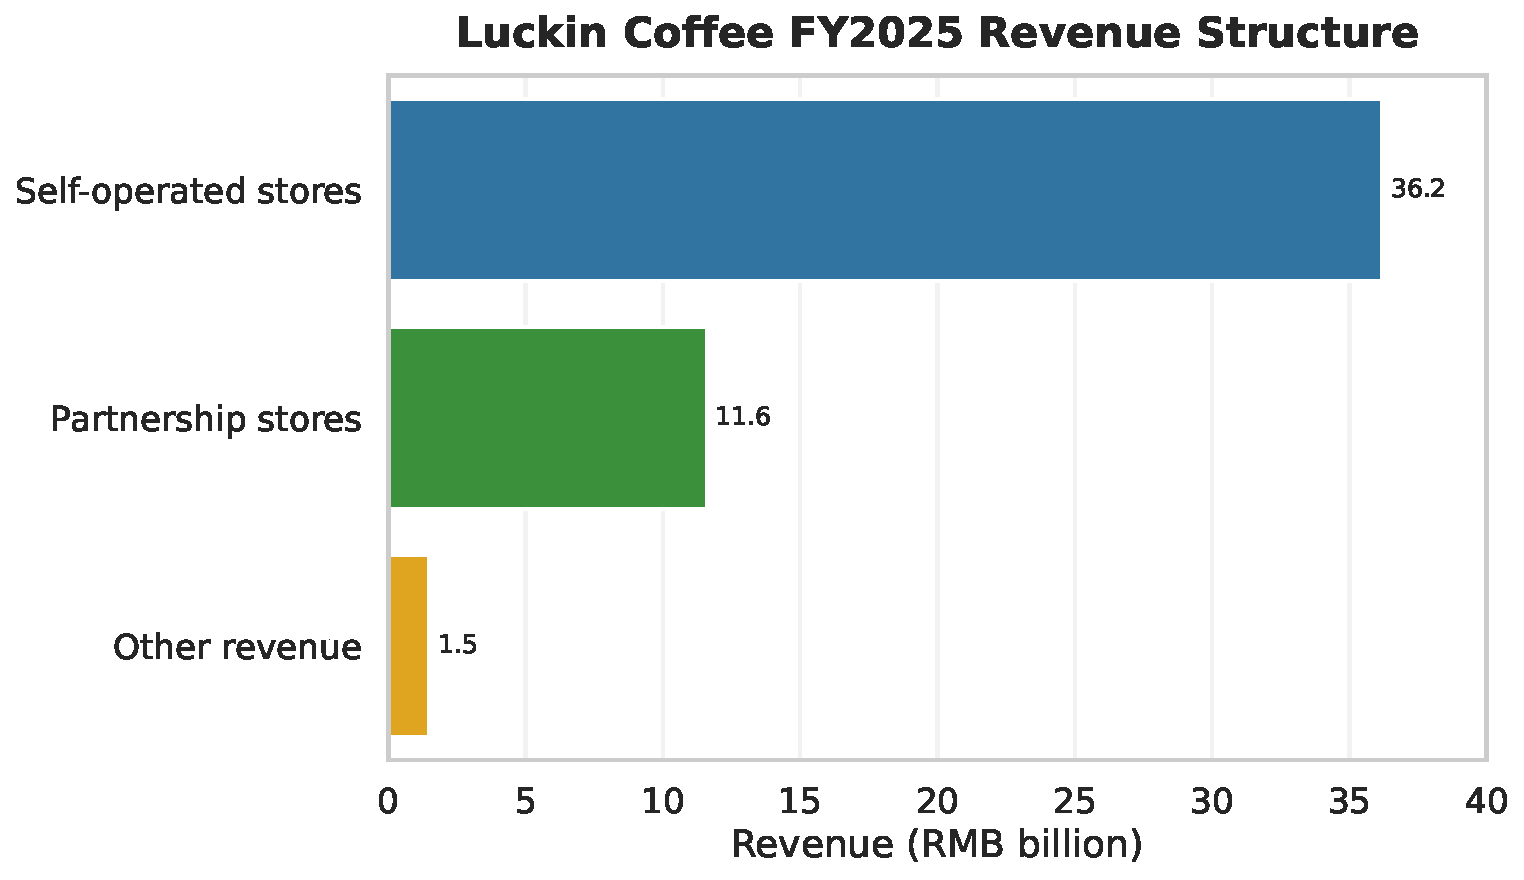
\includegraphics[width=0.78\textwidth]{fig_revenue_structure.pdf}
  \caption{Luckin Coffee FY2025 revenue structure. Source: Luckin Coffee FY2025 public disclosures~\cite{luckin2025annual,luckin2025results}.}
\end{figure}

\begin{figure}[H]
  \centering
  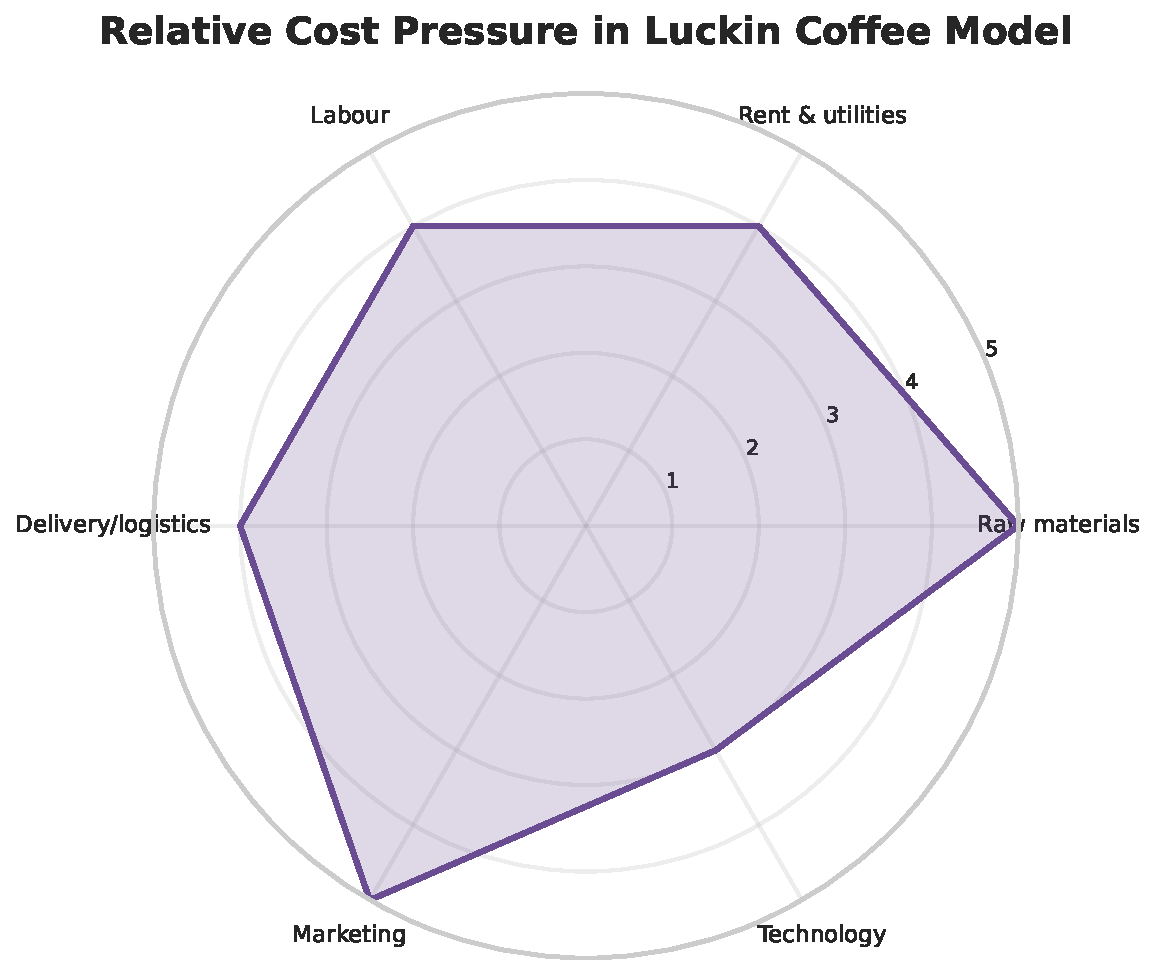
\includegraphics[width=0.64\textwidth]{fig_cost_pressure.pdf}
  \caption{Relative cost-pressure profile of Luckin Coffee's business model. Scores are qualitative assessments derived from case analysis.}
\end{figure}

The revenue chart highlights the centrality of self-operated stores, which remain the main revenue source and preserve operational control over brand experience and data capture. Partnership-store revenue, however, is strategically important because it supports asset-lighter geographic expansion. The cost-pressure profile shows why operational efficiency is central to the model: raw materials, promotional spending, delivery logistics, rent, and labour all interact with Luckin's affordability promise.

% =================== CONCLUSION ===================
\section{Conclusion}

The Balanced Scorecard and Business Model Canvas show that Luckin Coffee's competitive advantage is rooted in the alignment of strategy, technology, operations, and customer behaviour. Its financial mission depends on profitable scale; its customer mission depends on convenience and affordability; its internal process mission depends on standardised and data-integrated operations; and its learning and growth mission depends on continuous product innovation, employee capability, and digital infrastructure. The Business Model Canvas further demonstrates that Luckin captures value through a hybrid revenue structure while delivering value through a mobile-first, store-based fulfilment model. The two frameworks complement each other: the Balanced Scorecard decomposes strategic intent into measurable objectives, while the Business Model Canvas maps the structural logic of value creation and capture — together they set the stage for the enterprise architecture modelling and database design that follow.

\begingroup
\small
\setlength{\itemsep}{0pt}
\begin{thebibliography}{9}

\bibitem{luckin2025results}
Luckin Coffee Inc. (2026).
\emph{Luckin Coffee Announces Fourth Quarter and Fiscal Year 2025 Financial Results}.
\href{https://investor.luckincoffee.com/news-releases/news-release-details/luckin-coffee-announces-fourth-quarter-and-fiscal-year-2025/}{Luckin Coffee Investor Relations}.

\bibitem{luckin2025annual}
Luckin Coffee Inc. (2026).
\emph{Form 20-F Annual Report for the Fiscal Year Ended December 31, 2025}.
\href{https://www.sec.gov/Archives/edgar/data/1767582/000110465926035712/lk-20251231x20f.htm}{U.S. Securities and Exchange Commission}.

\bibitem{kaplan1992bsc}
Kaplan, R. S., \& Norton, D. P. (1992).
\emph{The Balanced Scorecard: Measures That Drive Performance}.
Harvard Business Review, 70(1), 71--79.

\bibitem{osterwalder2010bmg}
Osterwalder, A., \& Pigneur, Y. (2010).
\emph{Business Model Generation: A Handbook for Visionaries, Game Changers, and Challengers}.
John Wiley \& Sons.

\end{thebibliography}
\endgroup

\end{document}
